\documentclass{article}

% if you need to pass options to natbib, use, e.g.:
%     \PassOptionsToPackage{numbers, compress}{natbib}
% before loading neurips_2020

% ready for submission
% \usepackage{neurips_2020}

% to compile a preprint version, e.g., for submission to arXiv, add add the
% [preprint] option:
%     \usepackage[preprint]{neurips_2020}

% to compile a camera-ready version, add the [final] option, e.g.:
%     \usepackage[final]{neurips_2020}

% to avoid loading the natbib package, add option nonatbib:
     \usepackage[nonatbib]{neurips_2020}

\usepackage[utf8]{inputenc} % allow utf-8 input
\usepackage[T1]{fontenc}    % use 8-bit T1 fonts
\usepackage{hyperref}       % hyperlinks
\usepackage{url}            % simple URL typesetting
\usepackage{booktabs}       % professional-quality tables
\usepackage{amsfonts}       % blackboard math symbols
\usepackage{nicefrac}       % compact symbols for 1/2, etc.
\usepackage{microtype}      % microtypography
\usepackage{graphicx}  % <--- added
\usepackage{subcaption}
\usepackage{float}

\title{Summarization of instructional video transcripts using BERT}

% The \author macro works with any number of authors. There are two commands
% used to separate the names and addresses of multiple authors: \And and \AND.
%
% Using \And between authors leaves it to LaTeX to determine where to break the
% lines. Using \AND forces a line break at that point. So, if LaTeX puts 3 of 4
% authors names on the first line, and the last on the second line, try using
% \AND instead of \And before the third author name.

\author{%
  David S.~Hippocampus\thanks{Use  for providing further information
    about author (webpage, alternative address)---\emph{not} for acknowledging
    funding agencies.} \\
  Department of Computer Science\\
  Cranberry-Lemon University\\
  Pittsburgh, PA 15213 \\
  \texttt{hippo@cs.cranberry-lemon.edu} \\
  % examples of more authors
  % \And
  % Coauthor \\
  % Affiliation \\
  % Address \\
  % \texttt{email} \\
  % \AND
  % Coauthor \\
  % Affiliation \\
  % Address \\
  % \texttt{email} \\
  % \And
  % Coauthor \\
  % Affiliation \\
  % Address \\
  % \texttt{email} \\
  % \And
  % Coauthor \\
  % Affiliation \\
  % Address \\
  % \texttt{email} \\
}

\begin{document}

\maketitle

\begin{abstract}
In this paper, we study summarization of narrated instructional videos and various written texts. Unlike traditional video summarization which focuses on condensing select video frames, our work transfers unique step-by-step learning from written articles and videos to generate short summaries given video transcripts. We showcase how a top performing document-level encoder based on BERT can boost the fluency and generalizability of summaries across a wide variety of instructional text and videos. In addition to our fine tuning and ordered training methods, we present a novel dataset with over 5,000 transcripts extracted and constructed from open-domain videos and an online dataset written by different researchers. We demonstrate that our model is highly generalizable and produces summaries comparable to human written texts. To capture the semantic adequacy of our results, we use Content F1, Meteor, and human evaluations with a new framework that we designed for this project to score summaries.

\end{abstract}

\section{Introduction}
 
Google Insights states that how-to-videos are one of the most top watched videos on YouTube every year. Video content is rapidly growing and continues to be a prominent source for sharing information. With the increase in content, there has been a large demand for generating attractive content, keywords, and descriptions for marketing videos on such online platforms. Currently, many descriptions for video content are human written and configured to maximize results through search engine optimization. Our research attempts to address these issues by improving the semantic quality of short, textual summaries associated with such videos. We help contextualize videos by offering meaningful descriptions to enhance user engagement and experience.

Natural language processing tasks such as sentiment analysis, question and answering, and natural language generation have greatly advanced with the development of transformers and pre-trained models. Summarization, which is the task of condensing textual information into a short and concise form, has been improved on structured datasets. News articles and single documents are often used to enhance summary model performance. (citation). In abstractive video summarization, models which incorporate variations of LSTM and deep layered neural networks have become state of the art performers. More recently, multi-modal summarization, which combines speech, visual, and textual modalities seek to enhance summaries has emerged. However, the lack of human annotated data has limited the amount of benchmarked datasets available for such research. Additionally, most work in the field of video summarization has traditionally focused on the isolation and concatenation of important video frames using natural language processing techniques. Summarizing videos given conversational text is difficult to model. There are often inconsistencies and stylistic changes that are difficult to translate from spoken words. In this work, we challenge video summarizations by transferring top performing pretrained language models in single-document domains to that of open-domain videos.  

\section{Prior work}

\subsection{Text Summarization}

Text summarization is the task of generating shorter versions of documents while maintaining important information [need link]. This area of research in the natural language processing community has grown rapidly over the past several years due to its practical applications among various industries such as news, reviews, education. Summarization systems take two general approaches: extractive and abstractive. Extractive summarization provides users with textual summaries that have been copied and concatenated from important parts of a document. It is a reliable task capable of maintaining sentence structure and factual correctness. Abstract summarization generates a summary with content that is not always found in the underlying text. It is a complex task that mimics human summarization by generalizing and paraphrasing key points made in the document. 

Prior to 2014, summarization was centered on extracting lines from single documents using statistical models and neural networks had limited success[6, 7]. Sutskever et al. and Cho et al work on sequence to sequence models opened up new possibilities for neural networks in natural language processing. From 2014 to 2015, LSTMs (variety of RNN) became the dominant approach that achieved state of the art results. They became successful in tasks such as speech recognition, machine translation, parsing, image captioning, etc. It paved the way for abstractive summarization, which began to score competitively against extractive summarization. In 2017, Attention is all you need [8] provided a solution to the ‘fixed length vector’ problem, enabling neural networks to focus on important parts of the input for prediction tasks. Transformers with attention became more dominant for certain tasks [9].

\section{Problem Statement}

In our work we set a challenge to train a BERT-based model  that generates summaries from ASR (speech-to-text) scripts of competitive quality to human-curated descriptions on YouTube amateur narrated instructional . This challenge breaks down to the following low-level goals:
\begin{itemize}

\item Curate and publish a single source of truth data set of text and summaries aggregated and formatted from WikiHow articles, How2 videos, and CNN/DM stories;
\item Finetune existing BERT-based text summarization models to make them applicable to auto-generated scripts from instructional videos; 
\item Augment automated  metrics [Chin-Yew Lin] for evaluation of summaries with a framework for formalized expert assessment based on our research and criteria proposed by previous works.
\end{itemize}


 
\section{Methodology}

From the initial exploration and data analysis we saw that in the process of applying existing summarization models to Youtube video scripts  we will deal with challenges imposed by parsing speech-to-text output add more complexity to text summarization. For example, in one of the sample videos in our test data set closed captioning confuses the speaker’s words \emph{“how you get a text from a YouTube video”} for  \emph{“how you get attacks from a YouTube video”}. So, our work includes several iterations of the process described below:
\begin{itemize}
\item Collection and aggregation of data from multiple sources (HowTo video scripts, WikiHow, CNN stories, YouTube)
\item Preprocessing of video scripts to make them fit the text summarization models (e.g. errors in word recognition, lack of punctuation in closed captioning, getting rid of special characters etc., aligning inputs aggregated from multiple sources  to common format)
\item Text summarization models: selection, deployment, training,  and fine-tuning 
\item Experiments: applying models to the data and evaluation of the outputs using ROUGE metrics and human expert judgements
\end{itemize}
 
\subsection{Data Collection}
We hypothesized that the more labelled summarization data we bring, the more our model will benefit in the training process in terms of generalizability. 


\begin{itemize}

\item \textbf{CNN/Daily Mail dataset} provided by Hermann et. al 2015, the How2 Dataset, and Wikihow. The datasets illustrate different summary styles that range from single sentence phrases to short paragraphs. CNN and Daily Mail includes a combination of news articles and story highlights written with an average length of 119 words per article and 83 words per summary.
\item \textbf{Wikihow dataset}, a large scale text summarization containing over 200,000 single document summaries. Wikihow is a consolidated set of recent ‘How To’ instructional texts compiled from wikihow.com, ranging from topics such as ‘How to deal with coronavirus anxiety’ to ‘How to play Uno.’ The articles inside the dataset vary in size and topic but are structured to drive instructions across to the user. The first sentences of each paragraph are concatenated for form a summary for each article. 
\item \textbf{How2 Dataset} of 8,000 videos (approximately 2,000 hours). This YouTube compilation has videos averaging 90 seconds long and 291 word transcript length. It includes human written summaries where video owners were instructed to write with the interest of the viewer in mind. Summaries were two to three sentences in length with an average length of 33 words. 

\end{itemize}

Despite the development of instructional datasets such as Wikihow and How2, advancements in summarization have been limited by the availability of human annotated transcripts and summaries. Such datasets are difficult to obtain and expensive to create, often resulting in repetitive usage of singular-tasked and highly structured data . As seen in the How2 dataset, videos with a certain length and structured summary are used for training and testing. We introduce a new dataset, obtained from several How To and Do-It-Yourself youtube playlists and video sampling from the published HowTo100Million Dataset. The HowTo100Million Dataset is a large scale dataset of over 100 million video clips taken from narrated instructional videos across 140 categories. Our dataset incorporates a sample across all categories and utilizes the natural language annotations from automatically transcribed narrations provided by YouTube.

\begin{table}[H]
  \caption{DataSet}
  \label{dataset}
  \centering
  \begin{tabular}{llll}
    \toprule
  Dataset Size  &  5,195 (Youtube: 1,809. HowTo100Million: 3,386)    \\
 \midrule   
   YouTube Min/Max Length  &  4/1,940 words     \\
\midrule
YouTube Average Length & 259 words    \\
\midrule
  HowTo100Million Sample Min/Max Length & 5/6,587 words    \\
\midrule
HowTo100Million Sample Average Length & 859 words   \\
\bottomrule
  \end{tabular}
\end{table}

\subsection{Preprocessing}
\label{Preprocessing}

Due to diversity and complexity of our input data, a lot of our effort went into building a preprocessing pipeline out of blocks. The format of CNN/Daily Mail stories, wikiHow articles, and howTo scripts is different. We invested substantial efforts into converting them to a format that can be used. For the convenience of other researchers who may want to use similar methodology, we shared the results of aligning them to the same fromat that can be training. 

Another stream of work we have done at this stage is based on the heuristics observed during evaluation of results. Many scripts from YouTube (for the videos that we dupmed and HowTo100M dataset) have no punctuation, or it is not comprehensive. As a result, the model is misinterpreting text segment boundaries and produces low quality summaries or no summaries at all. With the help of Spacy library, we were able to fix this and restore sentence structures. 

We expected the differences in conversational style of the video scripts and writtent text of news stories (on which the models were pretrained) will impact quality of the output. In our first experiments with applying extractive summarization model that was pretrained on CNN/DM dataset, it manifested in a very distinct way. The model considered the first one-two sentences to be very important for summaries (this phenomena is referred to byt [15] as N-lead, where N is the number of important first sentences), and we ended up with getting many summaries looking like "hi!" and "hello, this is <first and last name>". It inspired us for implementing an improvement by using entity detection   \verb+spacy+ and \verb+nltk+ to remove introduction from the text that we feed to summarization model.  

The CNN/Daily Mail dataset has been preprocessed to remove news anchor introductions. For our Wikihow and How2 transcripts, we  did tokenization using the Stanford Core NLP toolkit and preprocessed the data in the same method used by (See et. al.).  


\subsection{Summarization models}

We used the BertSum model created by Yang trained on CNN and Daily Mail [Yang et. al.]  for our paper. This paper has 2 separate models for Extractive and abstractive summarization. Extractive summarization is generally a binary classification task with labels indicating whether sentences should be included in the summary. Abstractive summarization, on the other hand, requires language generation capabilities to create summaries containing novel words and phrases not found in the source text. 

The architecture in the Figure \ref{fig:architecure} shows the BERTSUM model. It uses a novel documentation level encoder based on BERT which can encode a document and obtain representation for the sentences. CLS token is added to every sentence instead of just 1 CLS token in the original BERT model. Abstractive model uses an encoder-decoder architecture, combining the same pretrained BERT encoder with a randomly initialized Transformer decoder. The model uses a special technique where the encoder portion is almost kept same with a very low learning rate and a separate learning rate is used for the decoder to make it learn better. 

\begin{figure}[H]
  \centering
  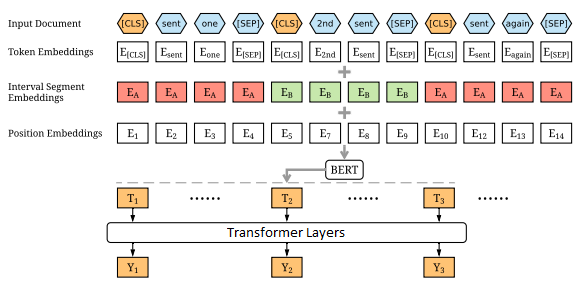
\includegraphics[scale=0.5]{bertsumarchitecture.png}
  \caption{BERTSUM Architecture. From [Yang et. al.]}
  \label{fig:architecure}
\end{figure}

We used a 4-GPU Linux machine and first trained on a small model with 10,000 steps using Extractive summarization in the beginning. Extractive summarization uses BERT base uncased and took around 12 hours to train. We fine tuned the whole model including the BERT layer. We established the baseline by training on 5,000 samples from the How2 dataset. We tuned few hyper parameters with different steps, batch sizes and epochs sizes. Then, we added CNN/Dailymail,full how2 dataset and 3,097 samples from Wikihow with a 50,000 step size to the training set and got better summaries. 

Finally, we used the Abstractive summarization model and all the datasets(CNN/DM, Wikihow and how2 datasets) with a total of 535527 examples and trained for 210,000 steps with a training batch size of 50 and more than 20 epochs in a specific order to get novel words and to get fluent summaries.This was done at the end as the abstractive model was very big and it took 4 days to train this model. These models were very demanding in terms of both memory and computational resources. The original model had more than 180 million parameters and had 2 Adam optimizers with $\beta_1$=0.9 and $\beta_2$ =0.999 for encoder and decoder respectively. Encoder used a learning rate of 0.002 and the decoder had a learning rate of 0.2. This was to make sure that the encoder was trained with more accurate gradients when the decoder was becoming stable.

\subsection{Scoring of resuls}
\label{Scoring}
We have observed examples of bad summaries with high ROUGE score, such as in Figure \ref{fig:funnysummary}, and good summaries with low ROUGE score. We believe that ROUGE is fine as a starting point for comparison, but the real evaluation of the output quality still requires human experts.

\begin{figure}[H]
  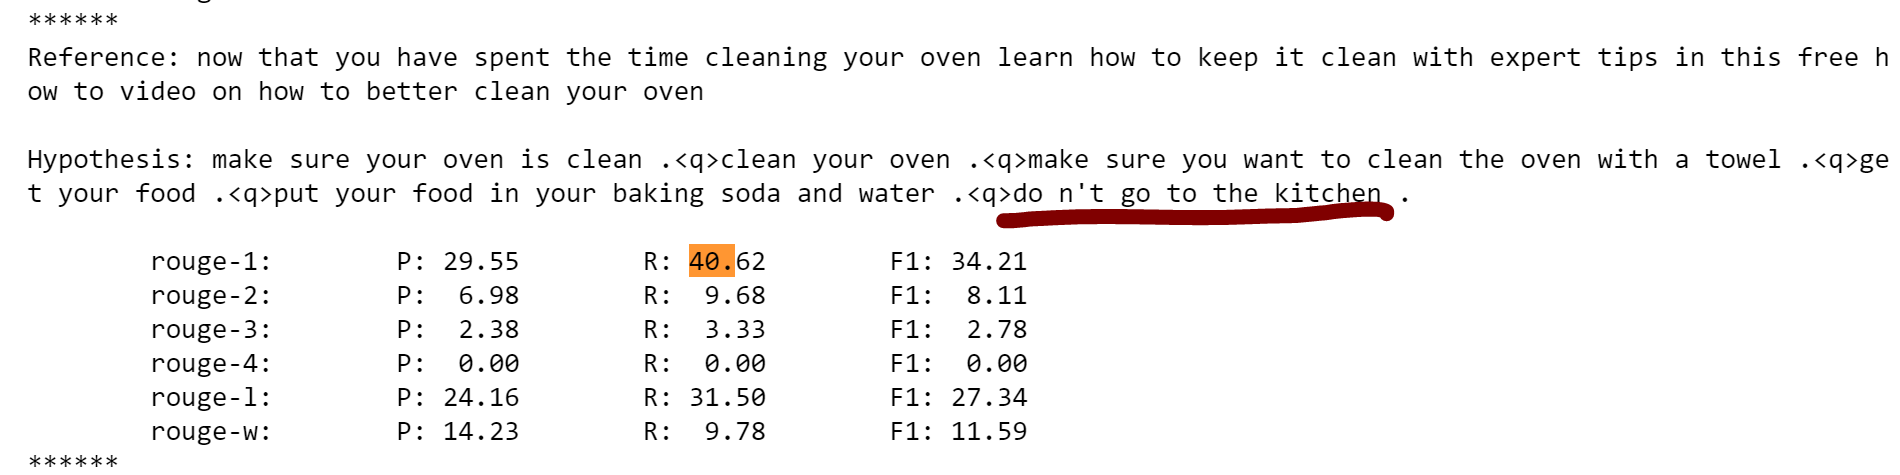
\includegraphics[width=\linewidth]{pic1.png}
  \caption{An example where ROUGE metric is confusing.}
  \label{fig:funnysummary}
\end{figure}

This is why we added another score to the rating -  Content F1, which was proposed in Carnegie Mellon university | to focus on the relevance of content. In calculation it is very similar to ROUGE, but discounts stop words and buzz words that frequently occur in the domain (in our case it was “learn from experts how to in this free online video”).  

In addition to automatically calculated scores, it is important to have human judges review the results. We have been doing this at all stages, but in addition to that we wanted to come up with a more formalized, objective and reusable process for engaging independent experts. In this effort we came up with a framework of criteria for evaluation that we implemented using Python, Google Forms, and Excel spreadsheets. Summaries for the surveys are randomly sampled to avoid biases.  In order to avoid leaking a hint about whether a summary was created by a human or our AI, we lower-cased all summaries, since the output of our model is uncased. We had two types of questions: one, a version of famous Turing test, was a challenge to distinguish AI from human-curated descriptions. Second was to give quality ratings to the summaries, so that we can see where to focus for further improvements. Below are definitions of criteria for clarity:
\begin{itemize}

\item Fluency: Does the text have a natural flow and rhythm?
\item Usefulness: Does it have enough information to make a user decide whether they want to spend time watching the video?
\item Succinctness: Does the text look concise or do does it have redundancy?
\item Consistency: Are there any ambiguous, confusing or contradicting statements in the text?
\item Realisticity: Is there anything that seems far-fetched and bizarre in words combinations, or do the statements look "normal"?

\end{itemize}

Options for grading of results are as follows: 1: Bad   2: Below Average   3: Average   4: Good   5: Great.



\section{Experiments and Results}

\subsection{Training}
Our baseline results were obtained from applying the state-of-the art extractive BertSum model pretrained on CNN/DailyMail. With the super power of BERT, we hoped to also see decent scores on howto videos, but that didn’t happen. Even more was our disappointment when we looked at the summaries the model generated: useless, confusing, and extremely funny, examples of which you can see in this slide. However, that experiment produced a ton of learnings: first, we saw that the model was doing relatively good on the health domain that is substantially covered in the news, and extremely poorly with topics like sports, arts, or culinary. Next, we realized that extractive summarization is not the right choice for our goal: that’s because most youtube videos are in very casual conversational style, while summaries have to be formal; so our only way is abstractive summarization, even though it’s harder. 

In order to create a generalizable abstractive model, we trained on large corpus of news. This allows our model to understand structured texts. We then introduced a comprehensive instructional text called Wikihow, which introduces the model to the how-to domain. Finally, we train and validate on the how-to dataset, narrowing the focus of the model to a selectively structured format. 

\begin{figure}[H]
\begin{subfigure}{.6\textwidth}
  \centering
  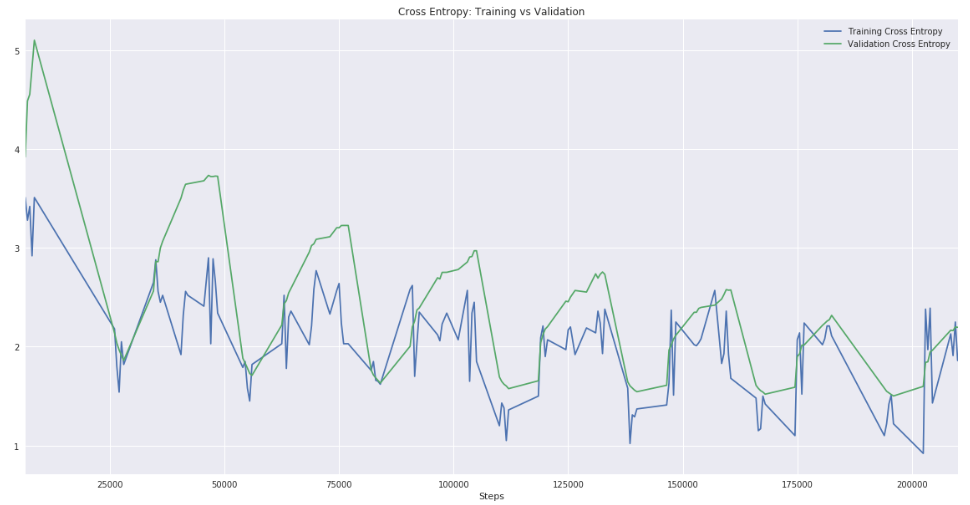
\includegraphics[width=\linewidth]{xent.png}
  \caption{Cross Entropy: Training vs Validation}
  \label{fig:xent}
\end{subfigure}%
\begin{subfigure}{.6\textwidth}
  \centering
  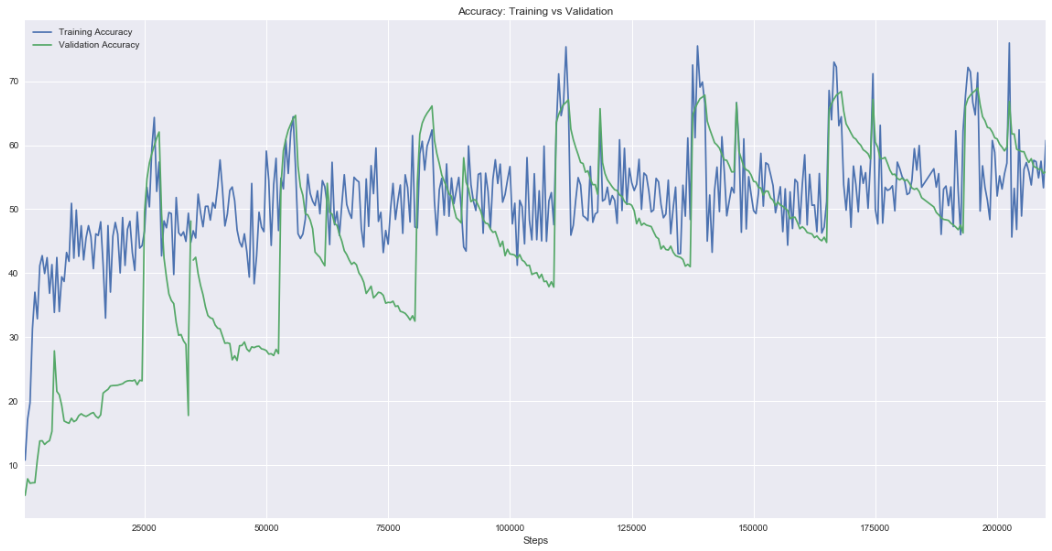
\includegraphics[width=\linewidth]{accuracy.png}
  \caption{Accuracy: Training vs Validation}
  \label{fig:accuracy}
\end{subfigure}
\caption{BertSum Abstractive Summarization: Model Performance}
\label{fig:modelperf}
\end{figure}

The cross entropy chart  in the Figure \ref{fig:xent} shows that the model is neither overfitting nor underfitting the training data. We want to see the lines meet and as seen here the model seems to be a good fit. Figure \ref{fig:accuracy} shows the model’s accuracy metric on the training and validation sets. The model is validated using the how2 dataset against the training dataset that includes all 4 sources. The model improves as expected with more steps(or epochs). 

\subsection{Evaluation}

The BertSum model created by Yang trained on CNN and Daily Mail [Yang] resulted in SOTA  scores when applied to samples from those datasets. However, when tested on our How2 Test dataset, it gave very poor performance and a lack of generalization in the model (see Table~\ref{table1}). Looking at the data, we found that the model tends to pick the first one or two sentences for the summary. This can be explained by the fact that the first paragraph of a news article often captures the gits of it, which the model learned. However, in the case of our instructional videos, the first sentences would be a non-informative introduction, such as "Hi there! My name is ...". Based on that, we hypothesized that removing introuductions from the text will help improve ROUGE scores. Indeed, we got a few points better after applying  preprocessing described in the Section \ref{Preprocessing} above. Yet another improvement came from adding word deduping at the output of the model, as we observed it occurring on the words that are rare and not known to the model, but we still couldn't get higher than 22.5 ROUGE-1 F1 and 20 ROUGE-L F1. Reviewing scores and texts of individual summaries showed that the model is doing better on some topics, such as medicine, and worse on others, such as sports. Again, this makes sense for a model that is trained on news: it isn't reasonable for it to be good with yoga-specific terminology, while news about health care are very common. In our next series of experiments, we used our own dataset for training.  Even though the difference in ROUGE scores for the results on [1-3] are not drastically different from [4-5], the quality of summaries from the perspective of human judges is qualitatively different.

Current best result was accomplished with leveraging the full set of labeled datasets (CNN/DM, WikiHow, and How2 videos) with order preserving configuration by setting shuffling parameter to false. We found that the order was very important: as human learner, the model wasn't able to make any substantial progress if it had to switch contexts between tasks of different complexity. The easiest training (CNN/DM) needs to be done first; then we move on to the next step of learning to summarize WikiHow, which covers more domains and has more complicated, but predictable structure; and only after that we proceed to video scripts, that present additional challenges of ad-hoc flow and conversational language. To our surprise, we didn't see big impact of spelling errors that frequently occur in ASR-generated scripts without human supervision, but ensuring correct boundaris between sentences by using Spacy to fix punctuation errors made a big difference. Our results for videos have reached the level of the best scores for news [1]. 

\begin{table}[H]
  \caption{Comparison of results}
  \label{table1}
  \centering
  \begin{tabular}{llll}
    \toprule
    \multicolumn{2}{c}{Experiment}                   \\
    \cmidrule(r){1-2}
    Model     & Pretraining Data     & Rouge-1 &Rouge-L\\
    \midrule
   1. BertSum  & CNN  and Daily Mail &18.08 &18.01    \\
 \midrule   
    2. BertSum with  & CNN  and Daily Mail & 20.51 &18.86     \\
      preprocessing    & & \\
\midrule
    3. BertSum with pre-     & CNN  and Daily Mail  & 22.47&20.07  \\
      and postprocessing    & & \\
\midrule
  4. BertSum  & How-To, WikiHow,   & 24.4 &21.45     \\
& CNN  and Daily Mail&\\
\midrule
  5. BertSum with  & How-To, WikiHow, & 26.32 &22.47    \\
postprocessing &CNN  and Daily Mail &\\
\midrule
 6. BertSum with  no shuffling& How-To, WikiHow, & 48.26 &44.02    \\
and more training data &CNN  and Daily Mail &\\
     \bottomrule
  \end{tabular}
\end{table}


From anecdotal paragraphs that made no sense, we went to very fluent and understandable video descriptions which give a clear idea about the content. However, our scores are not beating the scores from other researchers, even though we are using BERT and they had a mix of rule-based extractive and abstractive model running on much older engine. Closer look at comparison of the texts, though, showed that our summaries are in fluency and usefulness of summaries. Some examples are given below:

\begin{itemize}

\item Summary 1: growing rudbeckia requires full hot sun and good drainage. grow rudbeckia with tips from a gardening specialist in this free video on plant and flower care. care for rudbeckia with gardening tips from an experienced gardener
\item Benchmark 1: growing black - eyed - susan is easy with these tips, get expert gardening tips in this free gardening video .
\item Reference 1: growing rudbeckia plants requires a good deal of hot sun and plenty of good drainage for water . start a rudbeckia plant in the winter or anytime of year with advice from a gardening specialist in this free video on plant and flower care 
 
\item Summary 2: camouflage thick arms by wearing sleeves that are not close to the arms and that have a line that goes all the way to the waist. avoid wearing jackets and jackets with tips from an image consultant in this free video on fashion. learn how to dress for fashion modeling
\item Benchmark 2: hide thick arms and arms by wearing clothes that hold the arms in the top of the arm. avoid damaging the arm and avoid damaging the arms with tips from an image consultant in this free video on fashion .
\item Reference 2: hide thick arms by wearing clothes sleeves that almost reach the waist to camouflage the area .conceal the thickness at the top of the arms with tips from an image consultant in this free video on fashion.

\end{itemize}

Based on these observations, we decided that the model is mature enough for us move on to the final stage and leverage the power of independent experts and evaluate the quality of our summaries in comparison to descriptions that users provide for their videos on Youtube. We recruited a diverse group of 30 volunteers (27 have responded at the time of writing this paper) to blindly evaluate a set of 25 randomly selected video summaries  that were generated by our model and descriptions of videos on Youtube  from the dataset that we curated and HowTo100M (13 AI + 12 human-curated). We had two types of questions: one, a version of famous Turing test, was a challenge to distinguish AI from human-curated descriptions and used the framework described in Section \ref{Scoring}. You can see aggregated results for both evaluations in Figures \ref{fig:scores} - \ref{fig:quality}. We can see that nobody has been able to get 100\% accuracy in their Turing test answers, with many false positives and false negatives. This means that quality of the model output is comparable to average youtube summaries. Second, as we expected, the fluency of our summaries is almost as good as  human-curated text. Realisticity is the main growth opportunity, because the abstactive model makes up weird things, like “use chicken for an easy vegetarian recipe”.

\begin{figure}
\begin{subfigure}{.3\textwidth}
  \centering
  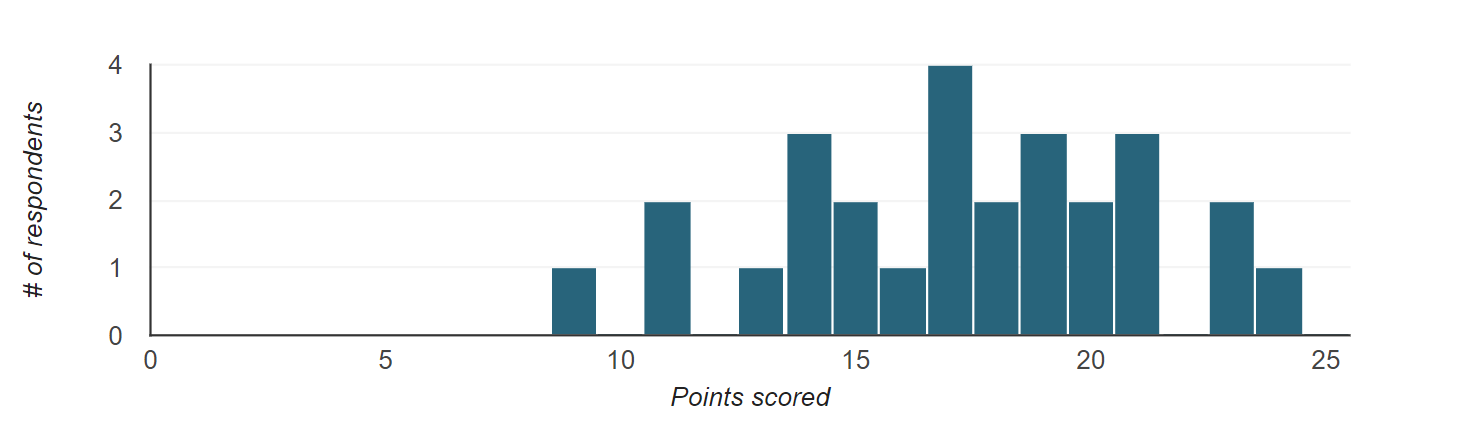
\includegraphics[width=\linewidth]{PointsScored.png}
  \caption{Turing test: Distinguish AI from Human summary result }
  \label{fig:scores}
\end{subfigure}
\begin{subfigure}{.3\textwidth}
  \centering
  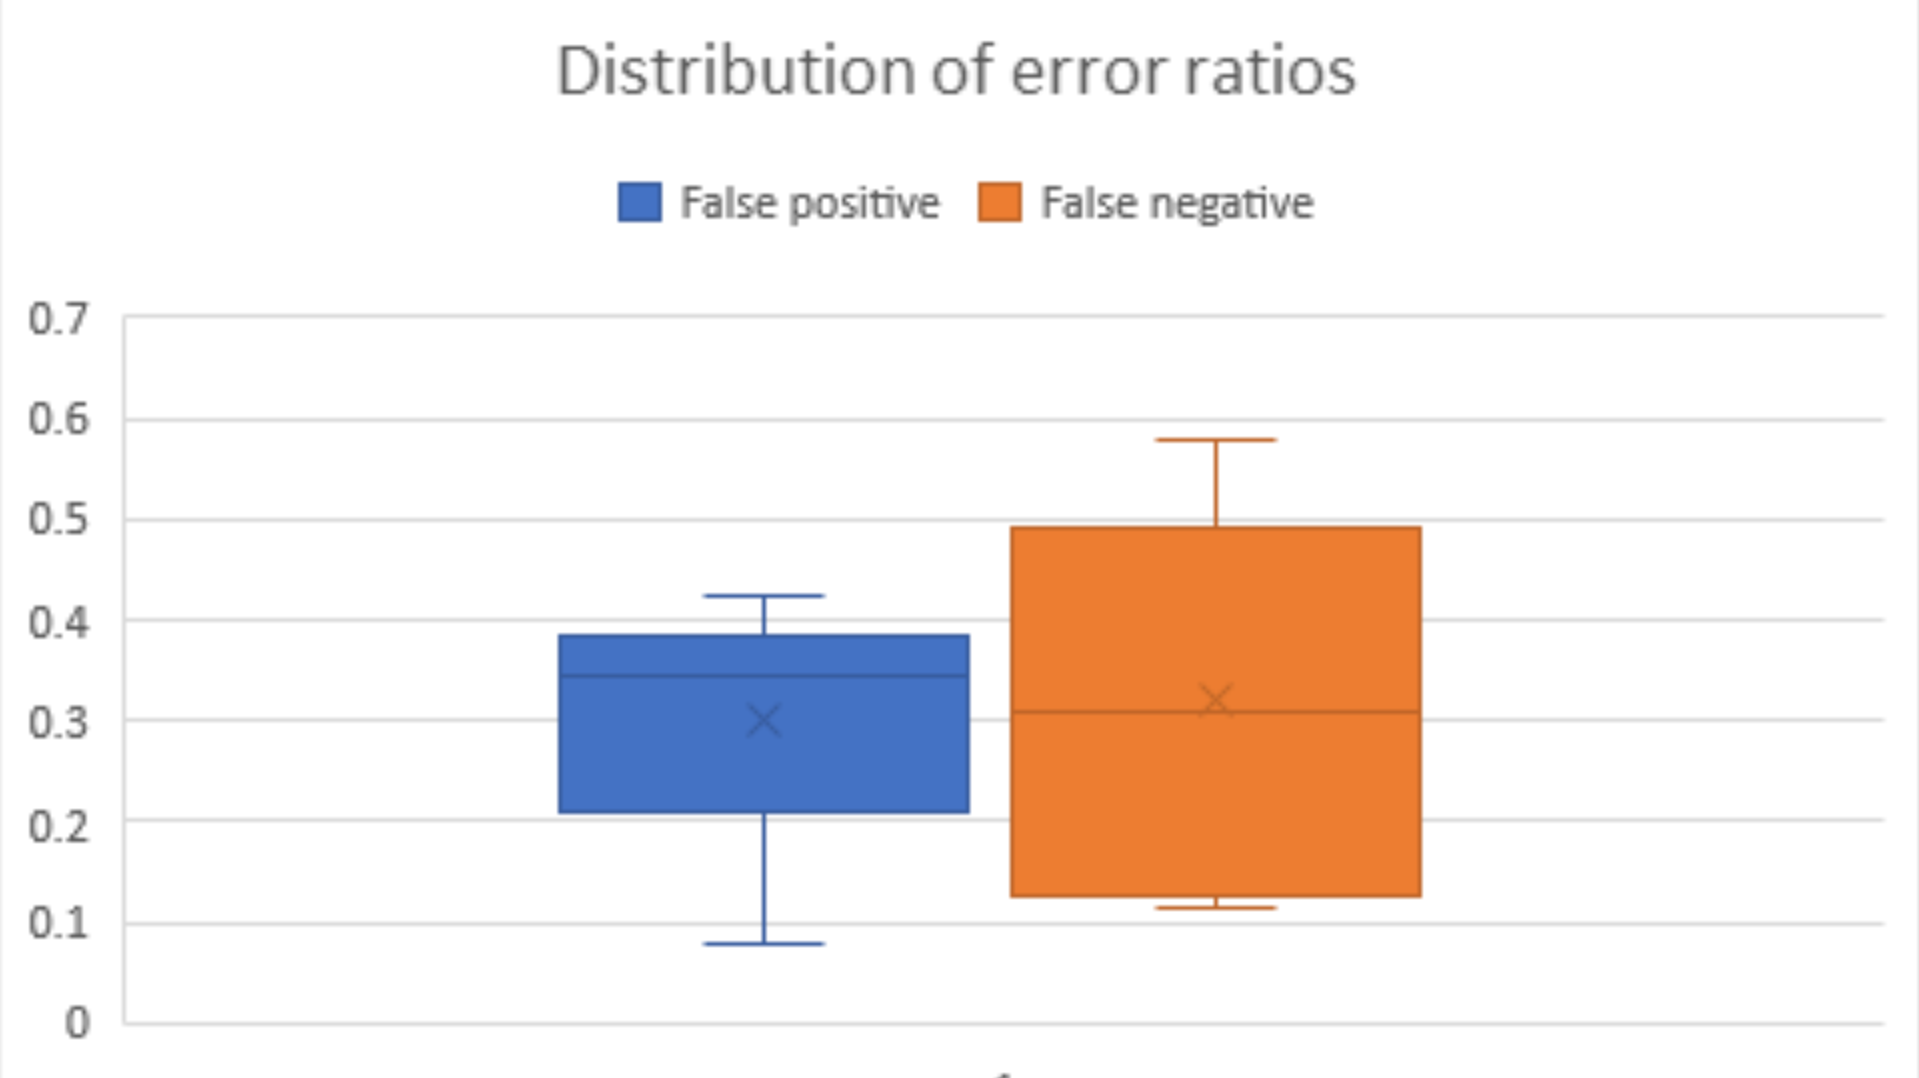
\includegraphics[width=\linewidth]{BoxPlots.png}
  \caption{Average FP (blue) and FN (orange) ratio per question}
  \label{fig:box}
\end{subfigure}
\begin{subfigure}{.3\textwidth}
  \centering
  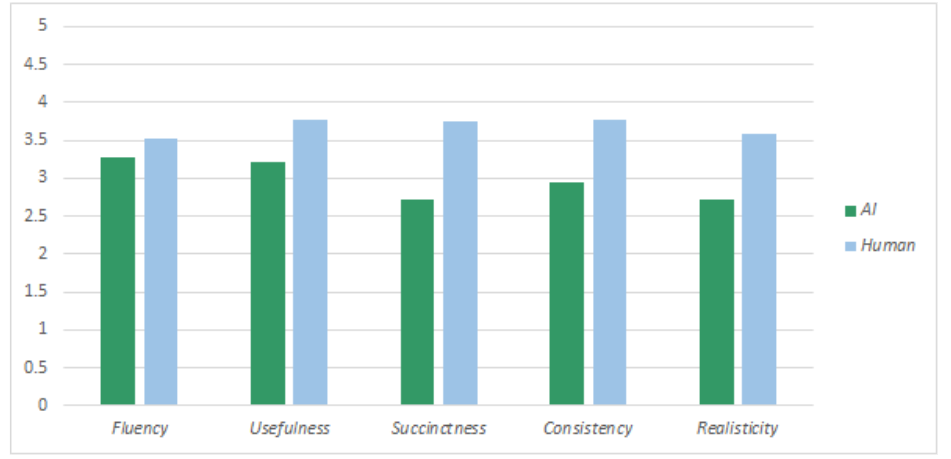
\includegraphics[width=\linewidth]{scores.png}
  \caption{Quality assessment of generated summaries}
  \label{fig:quality}
\end{subfigure}
\caption{Human evaluation of model-generated summaries in comparison with real video descriptions from YouTube}
\label{fig:survey}
\end{figure}


\section{Conclusion}

The contributions of our research are addressing multiple issues that we identified in pursuit of genaralizing BertSum model for summarization of instructional video scripts throughout the whole training process. 

\begin{itemize}

\item We complemented existing labeled summarization datasets with autogenerated instructional video scripts and human-curated descriptions 
\item We explored how different combinations of traing data and parameters  impact the training perfomance  of BertSum abstractive summarization model
\item We came up with novel preprocessing steps fpr auto-generated closed captioning scripts before summarization
\item We generalized BertSum abstractive summarization model to autogenerated instructional video scripts with the quality level that is close to randomly sampled descriptions created by Youtube users
\item We designed and implemented a new framework for blind unbiased review that produces more actionable and objective scores,  augmenting ROUGE, BLEU and Content F1
\end{itemize}
 
All the artifacts listed above are available  in to our repository for the benefit of future researchers \footnote{https://github.com/alebryvas/berk266/ - it's not a public repository yet, but we can provide access upon request}. Overall, the results we obtained by now on amateur narrated instructional videos  make us believe that we were able to come up with a trained model  that generates summaries from ASR (speech-to-text) scripts | of competitive quality to human-curated descriptions on YouTube. 

\section*{References} 

[1] Yang Liu, Mirella Lapata. Text Summarization with Pretrained Encoders.  \ (2019) URL. \url{https://arxiv.org/abs/1908.08345v2}

[2] Abigail See, Peter J. Liu, and Christopher D. Manning.\ (2017) Get to the point: Summarization with pointer-generator networks. In {\it Proceedings of the 55th Annual Meeting of the Association for Computational Linguistics \ (Volume 1: Long Papers)}, pages 1073-1083.

[3] Ilya Sutskever, Oriol Vinyals, and Quoc V Le. Sequence to sequence learning with neural networks.
 {\it Neural Information Processing Systems}, 2014. 

[4] Haoran Li, Junnan Zhu, Cong Ma, Jiajun Zhang, and Chengqing Zong. \ (2017). Multi-modal summarization for
asynchronous collection of text, image, audio and video. In {\it Proceedings of the 2017 Conference on Empirical
Methods in Natural Language Processing}, pages 1092–1102. Association for Computational Linguistics.

[5] Sanabria, R., Caglayan, O., Palaskar, S., Elliott, D., Barrault, L., Specia, L., and Metze, F. How2: A large-scale dataset for multimodal language understanding. {\it CoRR}, abs/1811.00347, 2018. URL. https://arxiv.org/abs/1811.00347

[6] Nenkova, A. (2005). Automatic text summarization of newswire: Lessons learned from the document understanding conference. In Proceedings of AAAI 2005, Pittsburgh, USA.

[7] Svore, K., Vanderwende, L., and Burges, C. (2007). Enhancing single-document summarization by combining RankNet and third-party sources. In Proceedings of the EMNLP-CoNLL, pages 448–457. [7, 8] 

[8] Yu-Hsiang Huang. Attention is all you need - pytorch. https://github.com/ jadore801120/attention-is-all-you-need-pytorch, 2018.

[9] Nima Sanjabi. Abstractive text summarization with attention-based mechanism. Master’s thesis, Universitat Politècnica de Catalunya, July 2018.

[10] Berna Erol, D-S Lee, and Jonathan Hull. 2003. Multimodal summarization of meeting recordings. In Multimedia and Expo, 2003. ICME’03. Proceedings. 2003 International Conference on, volume 3, pages III–25. IEEE.

[11] Dian Tjondronegoro, Xiaohui Tao, Johannes Sasongko, and Cher Han Lau. 2011. Multi-modal summarization of key events and top players in sports tournament videos. In Applications of Computer Vision (WACV), 2011 IEEE Workshop on, pages 471–478. IEEE

[12] Alexander M. Rush, Sumit Chopra, and Jason Weston. 2015. A neural attention model for abstractive sentence summarization. In Proceedings of the 2015 Conference on Empirical Methods in Natural Language Processing, pages 379–389. Association for Computational Linguistics.

[13] Shruti Palaskar, Jindrich Libovicky, Spandana Gella, Florian Metze. 2019. Multimodal Abstractive Summarization for How2 Videos. In Proceedings of the 57th Annual Meting of the Association for Computational Linguistics, pages 6587-6596. Association for Computational Linguistics.

[14] Antoine Miech, Dimitri Zhukov, Jean-Baptiste Alayrac, Makarand Tapaswi, Ivan Laptev, Josef Sivic. 2019. HowTo100M: Learning a Text-Video Embedding by Watching Hundred Million Narrated Video Clips. In ICCV 2019. https://arxiv.org/abs/1906.03327.
 
[15] TBA WikiHow
=======


\end{document}
